\input{../preamble.tex}

\lecturenumber{20}
\title{Locks}
\version{2.0.0}

\begin{document}
  \begin{frame}[plain, noframenumbering]
    \titlepage
  \end{frame}


	\begin{slide}

		\slidetitle{Our Next Complication}

		Let's create a program that spawns 8 threads

		\leftspace{}Each thread increments the same variable 10,000 times
		\medskip

		What should the final value of the variable be?

		\leftspace{}The initial value of the variable is 0
		\medskip

	\end{slide}
  
	\begin{slide}
  
		\slidetitle{Thread Racing}

		\vspace{-5mm}
	
		\begin{minted}{c}  
#define NUM_THREADS 8
static int counter = 0;

void* run(__attribute__((unused)) void* arg) {
    for (int i = 0; i < 10000; ++i) 
        ++counter;
    return NULL;
}
int main(void) {
    pthread_t thread[NUM_THREADS];
    for (int i = 0; i < NUM_THREADS; ++i)
        pthread_create(&thread[i], NULL, &run, NULL);
    for (i = 0; i < NUM_THREADS; ++i)
        pthread_join(thread[i], NULL);
    printf("counter = %i\n", counter);
    return 0;
}
		\end{minted}
  
  
	\end{slide}


	\begin{slide}
	
		\slidetitle{Aside / Review: What about processes?}
	
		\vspace{-5mm}
		\begin{minted}{c}  
#define NUM_PROCESSES 8
static int counter = 0;

int main(void) {
    for (int i = 0; i < NUM_PROCESSES; ++i) {
        pid_t pid = fork();
        if (pid == 0) {
            for (int j = 0; j < 10000; ++j) 
                ++counter;
            exit(0);
        }
    }
    for (int i = 0; i < NUM_PROCESSES; ++i) 
        wait(NULL);

    printf("counter = %d\n", counter);
    return 0;
}
		\end{minted}
	
	\end{slide}
	
	\begin{slide}
	
		\slidetitle{Bank Example}
		
		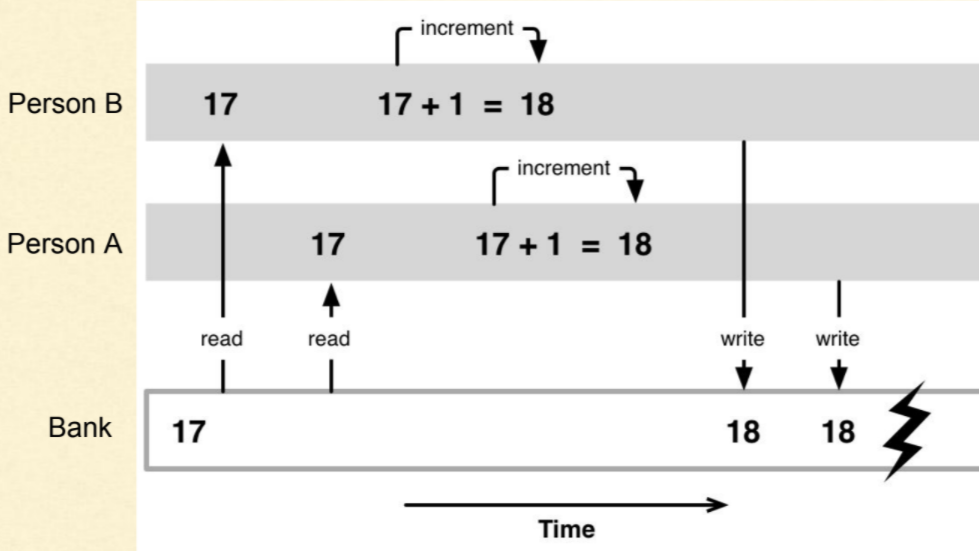
\includegraphics[width=100mm]{bank-example.png}
		
	\end{slide}
	
  \begin{slide}

    \slidetitle{Data Races Can Occur When Sharing Data}

    A data race is when two concurrent actions access the same variable

    and at least one of them is a write operation

  \end{slide}

  \begin{slide}

    \slidetitle{Atomic Operations are Indivisible}

    Any atomic instruction you may assume happens all at once
    \medskip

    This means you can not preempt it
    \medskip

    However, between two atomic instructions, you may be preempted

  \end{slide}

  \begin{slide}

    \slidetitle{Three Address Code (TAC) is Intermediate Code Used by Compilers}

    TAC is mostly used for analysis and optimization by compilers
    \medskip

    Statements represent one fundamental operation (assume each is atomic)

    \leftspace{}Useful to reason about data races and easier to read than assembly
    \medskip

    Statements have the form: $result := operand_1\:operator\:operand_2$

  \end{slide}

  \begin{slide}

    \slidetitle{GIMPLE is the TAC used by \texttt{gcc}}

    To see the GIMPLE representation of your compilation use:

    \leftspace{}{\tt -fdump-tree-gimple} flag
    \medskip

    To see all the three address code generated by the compiler (gcc) use:

    \leftspace{}{\tt -fdump-tree-all} flag
    \medskip

    GIMPLE is easier to reason about your code at a low-level without assembly

  \end{slide}

  \begin{slide}

    \slidetitle{Data Race}

    Instead of \texttt{count}, we'll look at \texttt{pcount} (the pointer to
    count, which is a global)
    \medskip

    The GIMPLE is the following:
    \begin{minted}{c}
D.1 = *pcount;
D.2 = D.1 + 1;
*pcount = D.2;
    \end{minted}
    \medskip
    
    Assuming that two threads execute this once each
    and initially \texttt{*pcount = 0}

    \leftspace{}What are the possible values of \texttt{*pcount}?

  \end{slide}

  \begin{slide}

    \slidetitle{Data Races}

    Let's call the read and write from thread 1 R1 and W1 (R2 and W2 from thread 2)
    \medskip

    We'll assume no re-ordering of instructions: always read then write in
    a thread
    \medskip

    All possible orderings:

	\begin{minipage}{0.25\textwidth}
	    \begin{minted}{c}
D.1 = *pcount;
D.2 = D.1 + 1;
*pcount = D.2;
		\end{minted}
	\end{minipage}
	\hfill
	\begin{minipage}{0.73\textwidth}
		\begin{center}
		  \begin{tabular}{llll|r}
			\multicolumn{4}{c|}{Order} & {\tt *pcount}\\
			\hline
			R1 & W1 & R2 & W2 &  \\
			R1 & R2 & W1 & W2 &  \\
			R1 & R2 & W2 & W1 &  \\
			R2 & W2 & R1 & W1 &  \\
			R2 & R1 & W2 & W1 &  \\
			R2 & R1 & W1 & W2 &  \\
		  \end{tabular}
		\end{center}
	\end{minipage}
	
  \end{slide}

    \begin{slide}

        \slidetitle{Locks: The Basic Idea}

	    \begin{minted}{c}
lock_t mutex; // A lock is just a variable
...
...
lock(&mutex); // Acquire the lock
count = count + 1
unlock(&mutex); // Release the lock
		\end{minted}
		\bigskip
	  
	    Only one thread can hold a lock at a time.
		\bigskip
		
		This thread is the owner of the lock.
	    \bigskip
	  
	    Other threads wait until the lock is free again.
  
    \end{slide}

	\begin{slide}
	
		\slidetitle{Pthread Locks}
		
\begin{minted}{c}
pthread_mutex_t lock = PTHREAD_MUTEX_INITIALIZER;

pthread_mutex_lock(&lock);
// protected code
pthread_mutex_unlock(&lock);
\end{minted}
    \medskip

    Everything within the {\tt lock} and {\tt unlock} is protected
    \medskip

    There's also a {\tt pthread\_mutex\_trylock} if needed

  \end{slide}

	\begin{slide}
	
		\slidetitle{Example of \texttt{pthread} lock}
		\vspace{-5mm}
\begin{minted}{c}
#define NUM_ITERATIONS 100000
int counter = 0;
pthread_mutex_t lock = PTHREAD_MUTEX_INITIALIZER;
void *worker(void *arg) {
    for (int i = 0; i < NUM_ITERATIONS; ++i) {
        pthread_mutex_lock(&lock);
        counter++;
        pthread_mutex_unlock(&lock);
    }
}
int main(void){
    pthread_t t1, t2;
    pthread_create(&t1, NULL, worker, NULL);
    pthread_create(&t2, NULL, worker, NULL);
    pthread_join(t1, NULL); pthread_join(t2, NULL);
    printf("Final counter value: %d\n", counter);
    return 0;
}
\end{minted}

	
	\end{slide}
	
	\begin{slide}
	
		\slidetitle{What could happen with locks}
		\vspace{-5mm}
		
\begin{minted}{c}
pthread_mutex_t a = PTHREAD_MUTEX_INITIALIZER;
pthread_mutex_t b = PTHREAD_MUTEX_INITIALIZER;
int main() {
    pthread_t x, y;
    pthread_create(&x, NULL, t1, NULL);
    pthread_create(&y, NULL, t2, NULL);
    pthread_join(x, NULL);
    pthread_join(y, NULL);
    return 0;
}
\end{minted}
	\medskip
	\begin{minipage}{0.45\textwidth}
	\begin{minted}{c}
void* t1(void* _) {
    pthread_mutex_lock(&a);
    pthread_mutex_lock(&b);  
    pthread_mutex_unlock(&b);
    pthread_mutex_unlock(&a);
    return NULL;
}
\end{minted}
	\end{minipage}
	\hfill
	\begin{minipage}{0.45\textwidth}
	\begin{minted}{c}
void* t2(void* _) {
    pthread_mutex_lock(&b);
    pthread_mutex_lock(&a);  
    pthread_mutex_unlock(&a);
    pthread_mutex_unlock(&b);
    return NULL;
}
\end{minted}
	\end{minipage}
	
	\end{slide}

  \begin{slide}

    \slidetitle{A Critical Section Means Only One Thread Executes Instructions}

    Safety (aka mutual exclusion)

    \leftspace{}There should only be a single thread in a critical section at
    once
    \medskip

    Liveness (aka progress)

    \leftspace{}If multiple threads reach a critical section, one must proceed

    \leftspace{}The critical section can't depend on outside threads

    \leftspace{}\leftspace{}You can mess up and deadlock (threads don't make progress)
    \medskip

    Bounded waiting (aka starvation-free)

    \leftspace{}A waiting thread must eventually proceed

  \end{slide}

  \begin{slide}

    \slidetitle{Critical Sections Should Also Have Minimal Overhead}

    Efficient

    \leftspace{}You don't want to consume resources while waiting
    \medskip

    Fair

    \leftspace{}You want each thread to wait approximately the same time
    \medskip

    Simple

    \leftspace{}It should be easy to use, and hard to misuse

  \end{slide}

	\begin{slide}
	
		\slidetitle{How do we build a lock?}
		
		How can we build an efficient lock?
		
	\end{slide}
	
  \begin{slide}

    \slidetitle{You Could Use a Lock to Implement Critical Sections}

    Assuming a uniprocessor operating system, your implementation could be:
    \medskip

    \begin{minted}{c}
void lock() {
  disable_interrupts();
}
void unlock() {
  enable_interrupts();
}   
    \end{minted}
    \medskip

    This would disable concurrency (assuming it ignores signals and interrupts)

    \leftspace{}This does not work on multiprocessors

  \end{slide}

  \begin{slide}

    \slidetitle{Let's Try to Implement a Lock in Software}

    \begin{minted}{c}
void init(int *l) {
  *l = 0;
}
void lock(int *l) {
  while (*l == 1);
  *l = 1;
}
void unlock(int *l) {
  *l = 0;
}   
    \end{minted}
    \medskip

    What's the issue with this implementation?

    \onslide<2->{\leftspace{}It's not safe (both threads can be in the critical section)}

    \onslide<2->{\leftspace{}It's not efficient, it wastes CPU cycles (busy wait)}

  \end{slide}

\begin{slide}

    \slidetitle{
      You Can Implement Locks in Software
      
      with Minimal Hardware
    }

    Your hardware requirements just have to ensure:
    \begin{itemize}
      \item Loads and stores are atomic
      \item Instructions execute in order
    \end{itemize}
    \medskip

    There are 2 main algorithms you could use:
    
    \leftspace{}\href{https://en.wikipedia.org/wiki/Peterson\%27s_algorithm}
    {Peterson's algorithm}
    and
    \href{http://en.wikipedia.org/wiki/Lamport\%27s_bakery_algorithm}
         {Lamport's bakery algorithm}
    \medskip

    However, they don't scale well, and processors execute
    out-of-order

  \end{slide}

  \begin{slide}

    \slidetitle{Let's Assume a Magical Atomic Function ---
                \texttt{compare\_and\_swap}}

    \texttt{compare\_and\_swap(int *p, int old, int new)} is atomic

    \leftspace{}It returns the original value pointed to

    \leftspace{}It only swaps if the original value equals \texttt{old}, and changes it to \texttt{new}
    \medskip

    Let's give it another shot:

    \begin{minted}[xleftmargin=1em]{c}
void init(int *l) {
  *l = 0;
}
void lock(int *l) {
  while (compare_and_swap(l, 0, 1));
}
void unlock(int *l) {
  *l = 0;
}   
    \end{minted}

  \end{slide}

  \begin{slide}

    \slidetitle{What We Implement is Essentially a Spinlock}

    Compare and swap is a common atomic hardware instruction
    \medskip

    On x86 this is the \texttt{cmpxchg} instruction (compare and exchange)
    \medskip

    However, it still has this ``busy wait'' problem
    \medskip

    Consider a uniprocessor system, if you can't get the lock, you should yield

    \leftspace{}Let the kernel schedule another process, that may free the lock
    \medskip

    On a multiprocessor machine, you could try again

  \end{slide}

  \begin{slide}

    \slidetitle{Let's Add a Yield}

    \begin{minted}{c}
void lock(int *l) {
  while (compare_and_swap(l, 0, 1)) {
    thread_yield();
  }
}
    \end{minted}

    Now we have a 
    \href{https://en.wikipedia.org/wiki/Thundering_herd_problem}{thundering herd}
    problem

    \leftspace{}Multiple threads may be waiting on the same lock
    \medskip

    We have no control over who gets the lock next

    \leftspace{}We need to be able to reason about it (FIFO is okay)

  \end{slide}

  \begin{slide}

    \slidetitle{We Can Add a Wait Queue to the Lock}

    \begin{minted}{c}
void lock(int *l) {
  while (compare_and_swap(l, 0, 1)) {
    // add myself to the lock wait queue
    thread_sleep();
  }
}
void unlock(int *l) {
  *l = 0;
  if (/* threads in wait queue */) {
    // wake up one thread
  }
}
    \end{minted}
    \medskip

    There are 2 issues with this:
    
    \begin{enumerate}
      \item lost wakeup, and
      \item the wrong thread gets the lock
    \end{enumerate}
  \end{slide}

  \begin{slide}

    \slidetitle{Lost Wakeup Example}

    \begin{minted}[linenos]{c}
void lock(int *l) {
  while (compare_and_swap(l, 0, 1)) {
    // add myself to the wait queue
    thread_sleep();
  }
}
void unlock(int *l) {
  *l = 0;
  if (/* threads in wait queue */) {
    // wake up one thread
  }
}
    \end{minted}
    \medskip

    Assume we have thread 1 (T1) and thread 2 (T2), thread 2 holds the lock

    \leftspace{}T1 runs line 2 and fails, swap to T2 that runs lines 10-12, T1
    runs lines 3 -4

    \leftspace{}\leftspace{}T1 will never get woken up!
  \end{slide}

  \begin{slide}

    \slidetitle{Wrong Thread Getting the Lock Example}

    \begin{minted}[linenos]{c}
void lock(int *l) {
  while (compare_and_swap(l, 0, 1)) {
    // add myself to the wait queue
    thread_sleep();
  }
}
void unlock(int *l) {
  *l = 0;
  if (/* threads in wait queue */) {
    // wake up one thread
  }
}
    \end{minted}
    \medskip

    Assume we have T1, T2, and T3. T2 holds the lock, T3 is in queue.

    \leftspace{}T2 runs line 9, swap to T1 which runs line 2 and succeeds

    \leftspace{}\leftspace{}T1 just stole the lock from T3!
  \end{slide}

  \begin{slide}

    \slidetitle{We Can Use Two Variables to Fix This (One to Guard)}

    \begin{columns}
      \begin{column}{0.5\textwidth}
        \begin{minted}{c}
typedef struct { int lock; int guard;
                 queue_t *q; } mutex_t;

void lock(mutex_t *m) {
  while (
    compare_and_swap(m->guard, 0, 1)
  );
  if (m->lock == 0) {
    m->lock = 1; // acquire mutex
    m->guard = 0;
  } else {
    enqueue(m->q, self);
    m->guard = 0;
    thread_sleep();
    // wakeup transfers the lock here
  }
}
        \end{minted}
      \end{column}
      \begin{column}{0.5\textwidth}
        \begin{minted}{c}
void unlock(mutex_t *m) {
  while (
    compare_and_swap(m->guard, 0, 1)
  );
  if (queue_empty(m->q)) {
    // release lock, no one needs it
    m->lock = 0; 
  }
  else {
    // direct transfer mutex
    // to next thread
    thread_wakeup(dequeue(m->q));
  }
  m->guard = 0;
}
        \end{minted}
      \end{column}
    \end{columns}

  \end{slide}

  \begin{slide}

    \slidetitle{There's STILL A Data Race}

    After a thread calls \texttt{lock}, it could get interrupted right before
    the \texttt{thread\_sleep}
    \medskip

    However, it's been added to the wait queue, so \texttt{thread\_wakeup}

    would try to wake up a thread that's not sleeping yet (we know it's about
    to)
    \medskip

    We could simply retry the call to \texttt{thread\_wakeup}

    until the thread finally calls \texttt{thread\_sleep}

  \end{slide}

  \begin{slide}

    \slidetitle{Remember What Causes a Data Race}

    A data race is when two concurrent actions access the same variable

    and at least one of them is a \textbf{write}
    \medskip

    We could have any many readers as we want

    \leftspace{}We don't need a mutex as long as nothing writes at the same
    time
    \medskip

    We need different lock modes for reading and writing

  \end{slide}

  \begin{slide}

    \slidetitle{Read-Write Locks}

    With mutexes/spinlocks, you have to lock the data,

    \leftspace{}even for a read since you don't know if a write could happen
    \medskip

    Reads can happen in parallel, as long as there's no write
    \medskip

    Multiple threads can hold a read lock ({\tt pthread\_rwlock\_rdlock}),

    \leftspace{}but only one thread may hold a write lock ({\tt pthread\_rwlock\_wrlock})

    \leftspace{}and will wait until the current readers are done

  \end{slide}

  \begin{slide}

    \slidetitle{We Can Use A Guard To Keep Track of Readers}

    \begin{columns}
      \begin{column}{0.5\textwidth}
        \begin{minted}{c}
typedef struct {
  int nreader;
  lock_t guard;
  lock_t lock;
} rwlock_t;

void write_lock(rwlock_t *l) (
  lock(&l->lock);
}

void write_unlock(rwlock_t *l) (
  unlock(&l->lock);
}
        \end{minted}
      \end{column}
      \begin{column}{0.5\textwidth}
        \begin{minted}{c}
void read_lock(rwlock_t *l) (
  lock(&l->guard);
  ++nreader;
  if (nreader == 1) { // first reader
    lock(&l->lock);
  }
  unlock(&l->guard);
}
void read_unlock(rwlock_t *l) (
  lock(&l->guard);
  --nreader;
  if (nreader == 0) { // last reader
    unlock(&l->lock);
  }
  unlock(&l->guard);
}
        \end{minted}
      \end{column}
    \end{columns}

  \end{slide}

  \begin{slide}
    \slidetitle{We Want Critical Sections to Protect Against Data Races}

    We should know what data races are, and how to prevent them:
    \begin{itemize}
      \item Mutex or spinlocks are the most straightforward locks
      \item We need hardware support to implement locks
      \item We need some kernel support for wake up notifications
      \item If we know we have a lot of readers, we should use a read-write lock
    \end{itemize}
  \end{slide}
  
\end{document}
